%! Author = sriadityavedantam
%! Date = 3/31/26

Generally, people denote that Algebraic Geometry is the study of the zero set of polynomials.
For example:

\begin{figure}[H]
    \centering
    \colorbox{white}{%
        \color{black}
        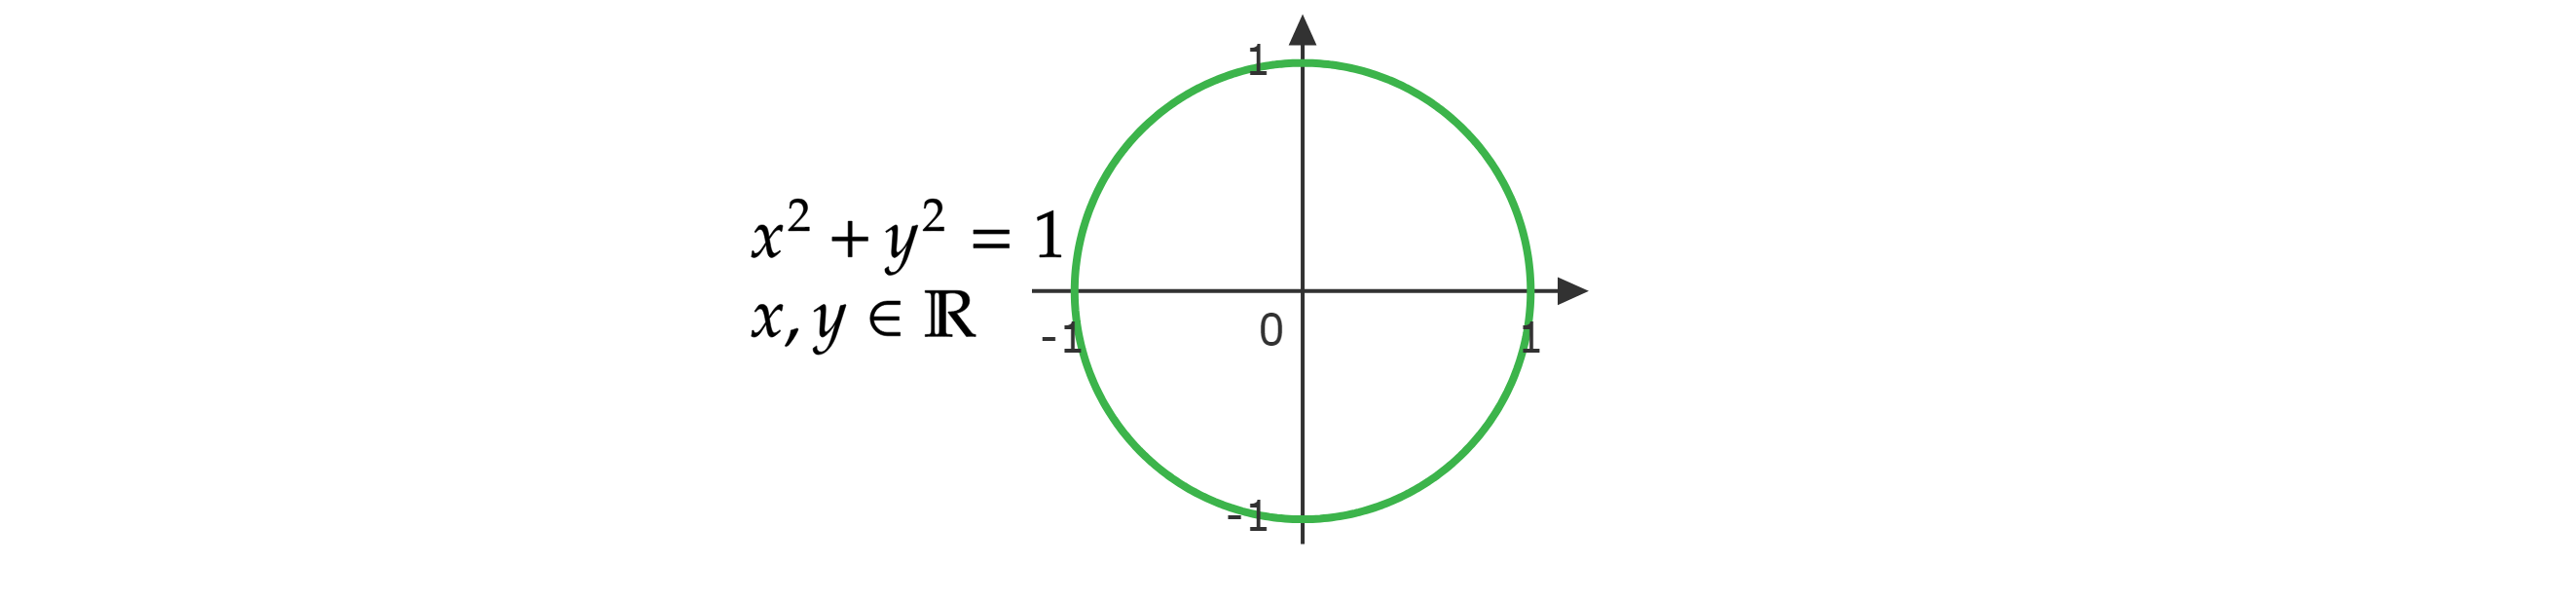
\includegraphics[width=\linewidth]{files/AlgebraicGeometry/images/circ1}
    }
    \caption{Unit Circle in the Reals}
\end{figure}

But we will be looking at solutions in specifically $\c$.

\section{Algebraic Curves of the Plane}

\begin{definition}[Affine Space]
    Let $\aa^n = \c^n$, which are n-tuples of complex numbers.
\end{definition}

For example we can have $(z_1,z_2)\in\c^2$ where $z_1,z_2\in\c$.
In fact, $\c[x_1,\ldots,x_n]$ is the polynomial algebra in n-variables.
If $f(x,y) = x^2 + y^2 - 1$, then $\{f = 0\}\subseteq\c^n = \aa^n$, or $\{x^2 + y^2 - 1 = 0\}$

\begin{definition}[Affine Plane Curve]
    In fact $f(x_1,x_2) = x_1^2 + x_2^2 - 1$, thus $\{f = 0 : x_1,x_2\in\c\}\subseteq \aa^2$, the affine plane, called an affine plane curve.
    Note that this curve is a $\rr-\dim(f) = 2$, but $\c-\dim(f) = 1$
\end{definition}

We often only plot the real component of affine plane curves.
But if $\aa = \c$, it is called an affine line, where $\cdim = 1$ and $\rdim = 2$, since we can create a complex number with two real numbers adjoined with $i$.This is due to the fact that if $y - x^2 = 0$, then we cannot draw a complex graph, but we can draw the real component as a parabola.

\begin{figure}[H]
    \centering
    \colorbox{white}{%
        \color{black}
        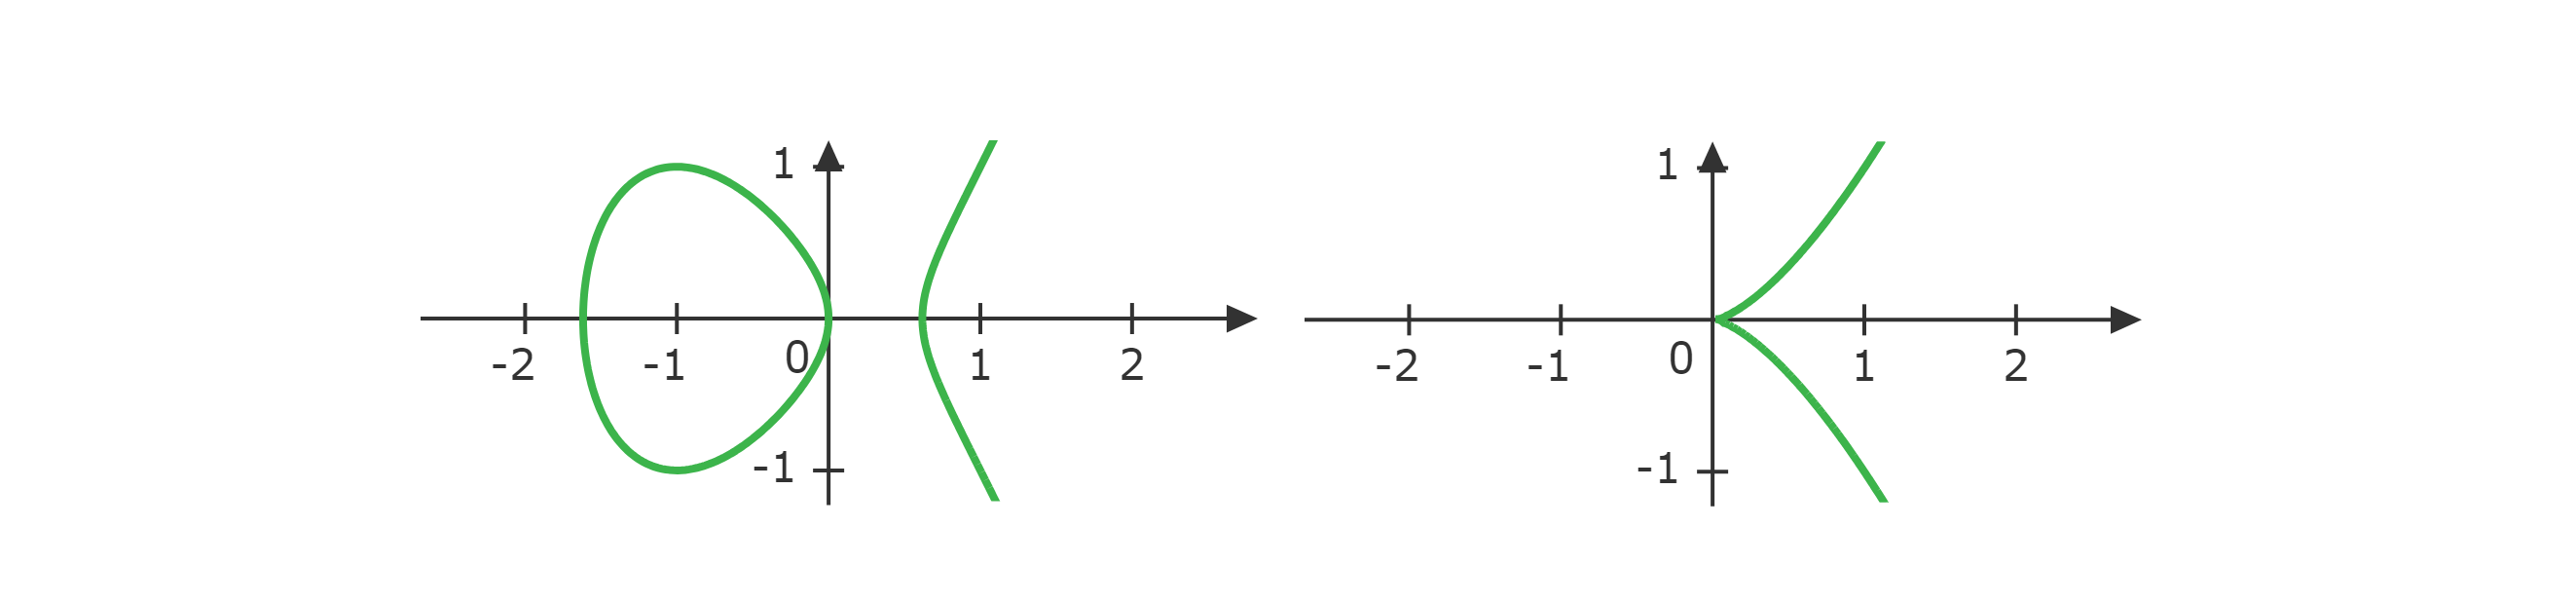
\includegraphics[width=\linewidth]{files/AlgebraicGeometry/images/graph}
    }
    \caption{Two Graphs of Real Components}
\end{figure}

\begin{definition}[Affine Algebraic Curve]
    $C$ is an affine curve defined by $\{f(x,y) = 0, x,y\in\c\}\subseteq\aa^2$.
\end{definition}

\begin{definition}[Degree of $C$]
    This is saying the same as the degree of $f$, which is the sum of the highest power in each variable.
\end{definition}

\[\deg(\{xy + x + y = 0\}) = 2\].
But all degree 2 affine plane curve polynomials are conics.

\begin{lemma*}{
    Every affine conic is of the form:
    \begin{enumerate}
        \item $x^2 - y^2 = 1$ (Hyperbola);
        \item $y = x^2$ (Parabola),
    \end{enumerate}
    which are equivalent by change of coordinates (basis).
}
\end{lemma*}

\begin{problem}{
    Show that ellipses can change into one of these forms.
}

\end{problem}

Throughout this course we will be working with algebraically closed fields, for example $\rr$ is not algebraically closed.

\begin{definition}[Algebraically Closed]
    If every non-constant polynomial has a root in the field.
\end{definition}

\begin{example}
    An example that $\rr$ is not closed is shown when
    \[
    \{x^2 + 1 = 0 : x\in\rr\} = \phi
    \]
    For any field, $\ff$, there exists $\bar{\ff}$ that is the smallest algebraically closed field containing $\ff$ called the algebraic closure of $\ff$.
    For example $\bar{\rr} = \c$.
\end{example}

\begin{proposition*}{
    Let $\kk$ be a arbitrary field, $f,g\in\kk[x,y]$ which are irreducible polynomials, meaning ti cannot be factored into non-constant. If $g$ is not divisible by $f$, then $f(x,y) = g(x,y) = 0$ by only finitely many satisfying solutions.
}
\end{proposition*}

We can easily understand the relationship between $\{f(x,y) = 0 : x,y\in\c\}\to C$, but what about the inverse direction. This is one of our goals in Algebraic Geometry. Given $C$, an algebraic curve which is irreducible, then we can understand its defining $\{f(x,y) = 0\}$ up to scalar.

\begin{definition}[Smooth Curve]
    A polynomial equation that is differentiable at all points.
\end{definition}

\begin{lemma*}{
    Any smooth affine conic is isomorphic to an affine plane curve.
}
\end{lemma*}

In fact, over $\rr$ any conic can be given by either a hyperbola, parabola, or ellipse; However, this is not true over the complexes. If we have $C\cong C^{'}$ as affine plane curves, then we can write the following commutative diagram:


\begin{figure}[H]
    \centering

    \tikzset{every picture/.style={line width=0.75pt}} %set default line width to 0.75pt

    \colorbox{white}{%
        \color{black}
        \begin{tikzpicture}[
            x=0.75pt,
            y=0.75pt,
            yscale=-1,
            xscale=1,
            every node/.style={text=black},
            every path/.style={draw=black},
            line width=0.75pt
        ]
%uncomment if require: \path (0,254); %set diagram left start at 0, and has height of 254

%Shape: Rectangle [id:dp5231215855668543]
            \draw   (357.87,43.93) -- (358.24,145.52) -- (321.18,145.65) -- (320.81,44.06) -- cycle ;


    % Text Node
            \draw (272,52) node [anchor=north west][inner sep=0.75pt]   [align=left] {C};
    % Text Node
            \draw (272,123) node [anchor=north west][inner sep=0.75pt]   [align=left] {C'};
    % Text Node
            \draw (328,49.4) node [anchor=north west][inner sep=0.75pt]    {$\mathbb{A}^{2}$};
    % Text Node
            \draw (328,122.4) node [anchor=north west][inner sep=0.75pt]    {$\mathbb{A}^{2}$};
    % Text Node
            \draw (295,52.4) node [anchor=north west][inner sep=0.75pt]    {$\hookrightarrow $};
    % Text Node
            \draw (295,121.4) node [anchor=north west][inner sep=0.75pt]    {$\hookrightarrow $};
    % Text Node
            \draw (274,85.4) node [anchor=north west][inner sep=0.75pt]    {$\downarrow $};
    % Text Node
            \draw (328,84.4) node [anchor=north west][inner sep=0.75pt]    {$\downarrow $};
    % Text Node
            \draw (265,88.4) node [anchor=north west][inner sep=0.75pt]    {$\cong $};
    % Text Node
            \draw (335,88.4) node [anchor=north west][inner sep=0.75pt]    {$\cong $};
    % Text Node
            \draw (305,107.68) node [anchor=north west][inner sep=1.3pt]  [rotate=-225.62]  {$\circlearrowright $};
    % Text Node
            \draw (363,74) node [anchor=north west][inner sep=0.75pt]   [align=left] {\begin{minipage}[lt]{57.72pt}\setlength\topsep{0pt}
                \begin{center}
                    Change in\\Coordinates
                \end{center}

            \end{minipage}};
    % Text Node
            \draw (235,161.4) node [anchor=north west][inner sep=0.75pt]    {$\begin{bmatrix}
                                                                                  x^{'} \\
                                                                                  y^{'}
            \end{bmatrix} =\begin{bmatrix}
                               M
            \end{bmatrix}_{2x2}\begin{bmatrix}
                                   x\\
                                   y
            \end{bmatrix} +\begin{bmatrix}
                               T
            \end{bmatrix}_{2x1}$};


        \end{tikzpicture}
    }
    \caption{Isomorphism of Affine Curves through Change in Basis}
\end{figure}

If we take the following conic $C: \{f(x,y) = x^2 + y^2 - 1 = 0\}$, which is a circle, then we can translate it to a conic in the complexes by:
\begin{align*}
    x &\mapsto x\\
    y &\mapsto iy\\
    x^2 + y^2 - 1 &\mapsto x^2 - y^2 - 1
\end{align*}